% !TEX root = Master.tex

In this chapter, we will deep dive into various ways on how to actually model, evaluate and interpret the dependence structure of different hierarchy levels. We first start at key category cluster level and compare the capabilities of the tried and tested methods on article unit sales. \\

One side note on the promotion intensities of Black Friday and Friends \& Family (see \autoref{tab:transactional_data}) is that on higher levels such as key category cluster, as we aggregate our data, promotion intensities become binary values indicating whether the respective promotion took place in those respective weeks. Also note that Black Friday and Friends \& Family weeks do not overlap. When we aggregate our data, not only promotion intensities need to be adapted. In the course of this, we average the total markdown percentage of all articles belonging to a respective aggregation group, e.g. each key category cluster obtains its own mean total markdown percentage. However, when we are trying to model dependence measures as functions of covariates, we need a unifying feature for such groups. Luckily, we can readily average the aggregated total markdown percentages. \autoref{fig:total_markdown_pct_kcc} clarifies the strong linear correlations of those aggregated markdown percentages, therefore this simple solution should be rational. \\


\begin{figure}[H]
\centering
  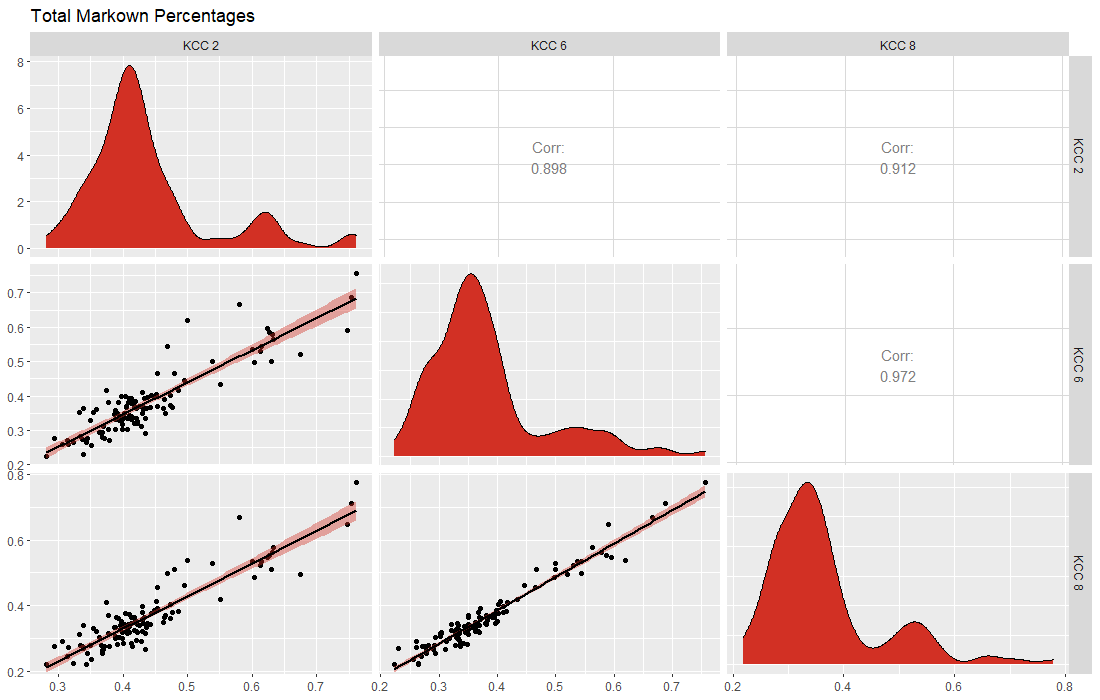
\includegraphics[width=0.8\linewidth]{figures/total_markdown_pct_kcc.png}
  \caption{Pairwise total markdown percentages of key category clusters}
  \label{fig:total_markdown_pct_kcc}
\end{figure}

Another important aspect of the modelling part is that usually, continuous responses are implied in the literature. Nevertheless, discrete responses (like in our "real" case) are also justified when explanatory variables are involved. A nice explanation can be found in \cite{trivedi2017note}.


